\documentclass{article}

\usepackage{arxiv}

\usepackage[utf8]{inputenc} % allow utf-8 input
\usepackage[T1]{fontenc}    % use 8-bit T1 fonts
\usepackage{hyperref}       % hyperlinks
\usepackage{url}            % simple URL typesetting
\usepackage{booktabs}       % professional-quality tables
\usepackage{amsfonts}       % blackboard math symbols
\usepackage{nicefrac}       % compact symbols for 1/2, etc.
\usepackage{microtype}      % microtypography
\usepackage{lipsum}
\usepackage{graphicx}

\usepackage{listings}
\usepackage{xcolor}

\definecolor{codegreen}{rgb}{0,0.6,0}
\definecolor{codegray}{rgb}{0.5,0.5,0.5}
\definecolor{codepurple}{rgb}{0.58,0,0.82}
\definecolor{backcolour}{rgb}{0.95,0.95,0.92}

\lstdefinestyle{mystyle}{
    backgroundcolor=\color{backcolour},   
    commentstyle=\color{codegreen},
    keywordstyle=\color{magenta},
    numberstyle=\tiny\color{codegray},
    stringstyle=\color{codepurple},
    basicstyle=\ttfamily\footnotesize,
    breakatwhitespace=false,         
    breaklines=true,                 
    captionpos=b,                    
    keepspaces=true,                 
    numbers=left,                    
    numbersep=5pt,                  
    showspaces=false,                
    showstringspaces=false,
    showtabs=false,                  
    tabsize=2
}

\lstset{style=mystyle}

\graphicspath{ {./images/} }

\title{Sentiment analysis su dataset IMDB}

\author{
 Matteo Galiazzo \\
  Dipartimento di Informatica - Scienza e Ingegneria\\
  Università di Bologna\\
  \texttt{matteo.galiazzo@studio.unibo.it} \\
  %% examples of more authors
%    \And
%  Zixuan Lu \\
%   School of Coumputing and Information\\
%   University of Pittsburgh\\
%   Pittsburgh, PA 15213 \\
%   \texttt{ZIL50@pitt.edu} \\
%   \And
%  Yuchen Lu \\
%   School of Coumputing and Information\\
%   University of Pittsburgh\\
%   Pittsburgh, PA 15213 \\
%   \texttt{yul217@pitt.edu} \\
  %% \AND
  %% Coauthor \\
  %% Affiliation \\
  %% Address \\
  %% \texttt{email} \\
  %% \And
  %% Coauthor \\
  %% Affiliation \\
  %% Address \\
  %% \texttt{email} \\
  %% \And
  %% Coauthor \\
  %% Affiliation \\
  %% Address \\
  %% \texttt{email} \\
}

\begin{document}
\maketitle
\begin{abstract}
TODO
\end{abstract}

% keywords can be removed
%\keywords{First keyword \and Second keyword \and More}


\section{Introduction}

This project presents an implementation of sentiment analysis on the IMDB movie reviews dataset using deep learning approaches.
The project explores two different Long Short-Term Memory (LSTM) architectures: a standard LSTM and a bidirectional LSTM model.
The implementation leverages TensorFlow and Keras for model development and training, with the goal of accurately classifying movie reviews as either positive or negative.

\subsection{Recurrent Neural Networks}

The problem of using a MLP or CNN to process text is the fact that we have a fixed input.
This means that if we use one of this architectures we are constrained by a fixed window for our input.
For solving this problem scholars introduced Recurrent Neural Networks (RNNs).
In a RNN we have a sequence of words $x_1, ..., x_n$.
To process this sequence we inject $x_1$ in the hidden layer and output $o_1$.
The information of $x_2$ is processed together with the output of the previous computation.
So in principle when you compute the output of $x_n$ you take into consideration all the previous output.
This way the sequence length is independent from the network structure.

Two very common memory cells for RNNs are Long Short-Term Memory (LSTM) or Gated Recurrent Units (GRU).
RNNs have a problem. They can only see the past of the sequence.

\begin{figure}[htbp]
  \centering
  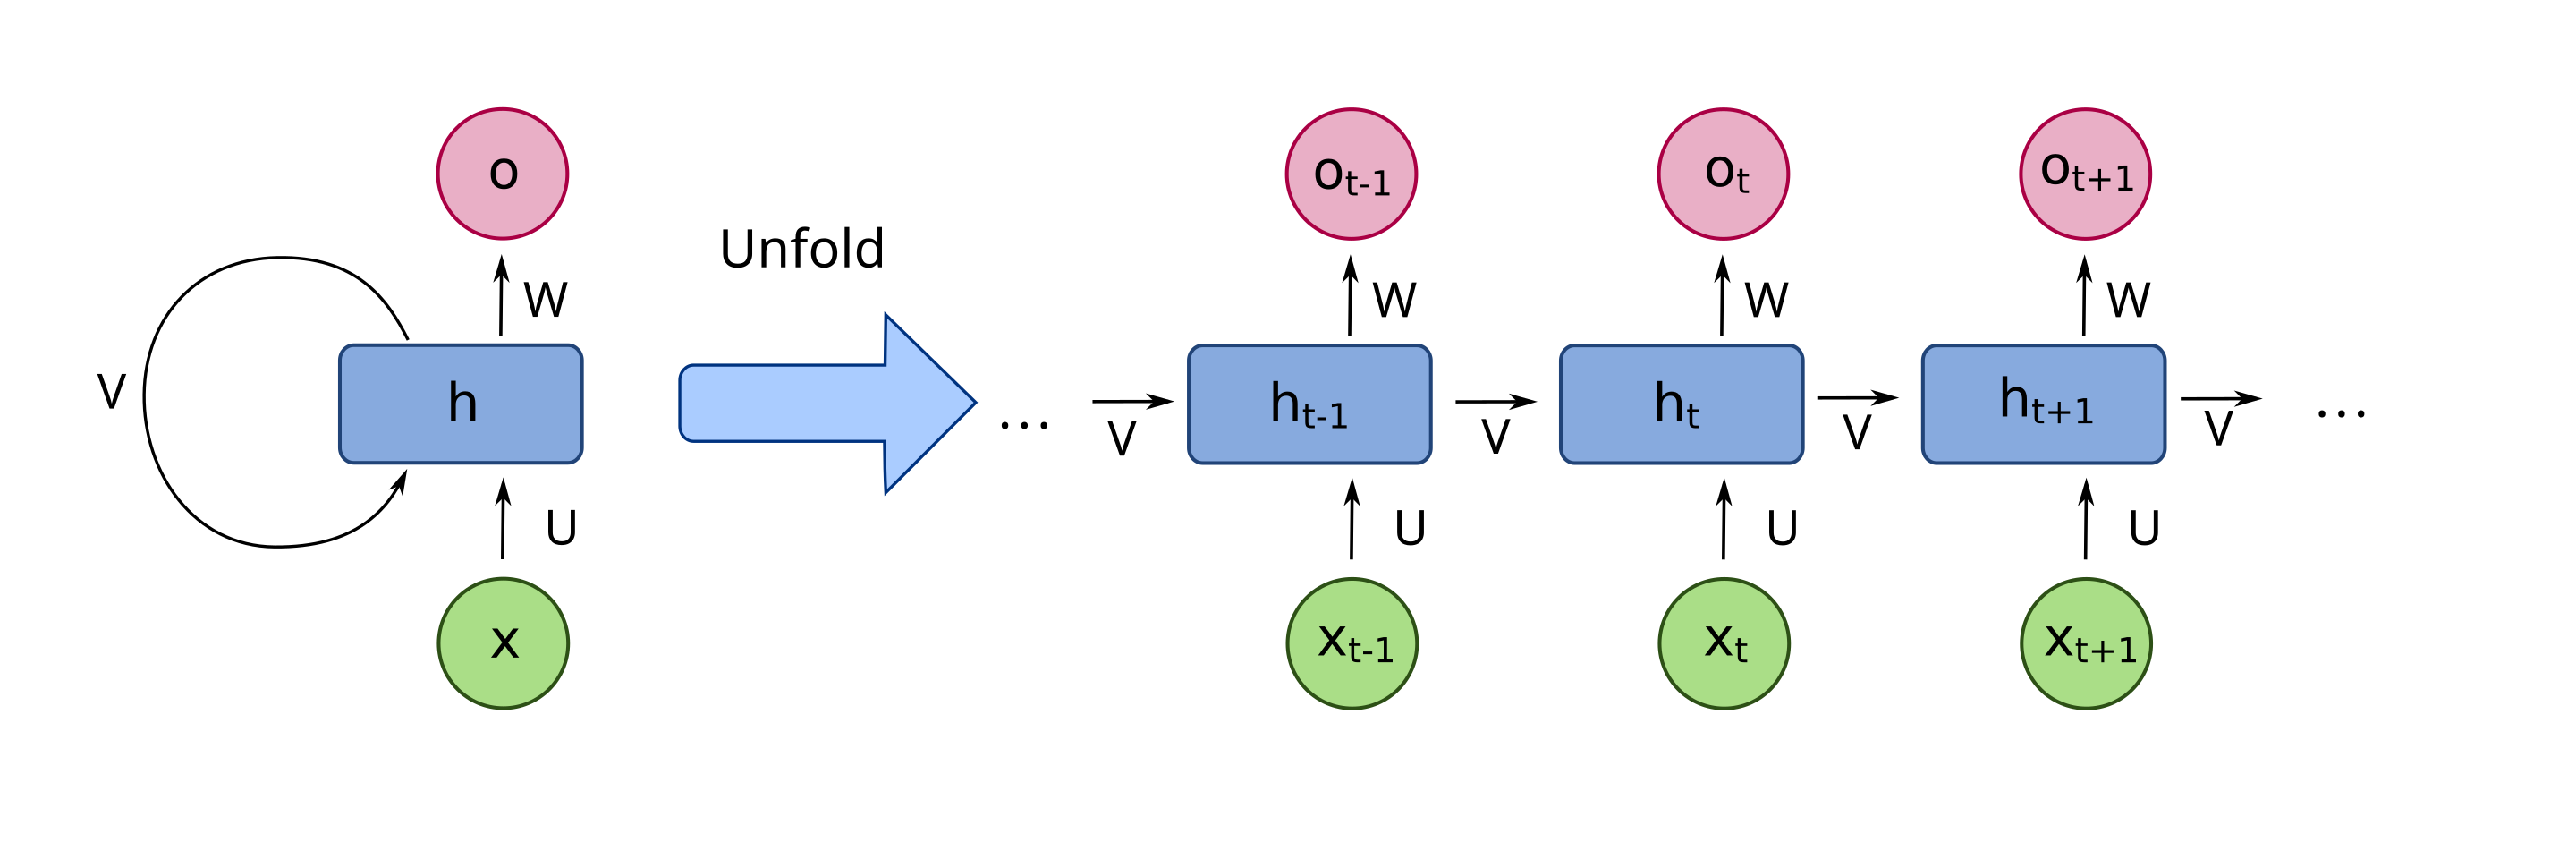
\includegraphics[width=0.8\linewidth]{img/rnn_unfolded.png}
  \caption{A compressed (left) and unfolded (right) RNN}
  \label{fig:rnn_unfolded}
\end{figure}

Abstractly speaking, an RNN is a function $f_{\theta}$ of type $(x_t, h_t) \rightarrow (y_t, h_{t+1})$, where:
\begin{itemize}
  \item $x_t$: input vector.
  \item $h_t$: hidden vector.
  \item $y_t$: output vector.
  \item $\theta$: neural network parameters.
\end{itemize}

It's a neural netowrk that maps an input $x_t$ into an output $y_t$, with the hidden vector $h_t$ playing the role of "memory", a partial record of all previous input-output pairs.
At each step, it transforms input to an output, and modifies its "memory" to help it to better perform future processing.

The figure \ref{fig:rnn_unfolded} may be misleading to many because practical neural netowrk topologies are frequently organized in "layers" and the drawing gives that appearance.
However, what appears to be layers are, in fact, different steps in time, "unfolded" to produce the appearance of layers.

\subsubsection{Bidirectional RNNs}

We can combine two RNNs, one processing the input sequence in one direction, and the other one in the opposite direction
This is called a bidirectional RNN, and it's structured as follows:
\begin{itemize}
  \item The forward RNN processes in one direction: $f_{\theta}(x_0, h_0) = (y_0, h_1), f_{\theta}(x_1, h_1) = (y_1, h_2), ...$
  \item The backward RNN processes in the opposite direction:
  
  ${f'}_{\theta '}(x_N, {h'}_N) = ({y'}_N, {h'}_{N-1}), {f'}_{\theta '}(x_{N-1}, {h'}_{N-1}) = ({y'}_{N-1},{h'}_{N-2}), ...$
\end{itemize}

The two output sequences are then concatenated to give the total output: $((y_0, {y'}_0), (y_1, {y'}_1), ..., (y_N, {y'}_N))$.
Bidirectional RNN allows the model to process a token both in the context of what came before it and what came after it.

\begin{figure}[htbp]
  \centering
  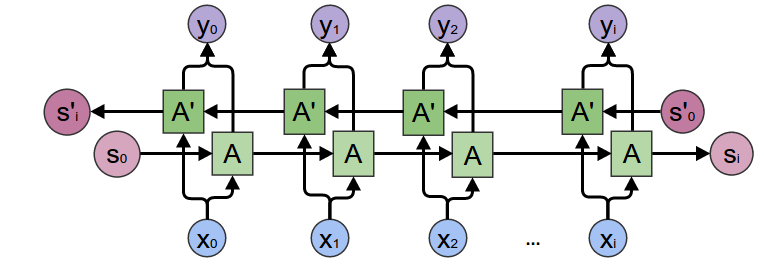
\includegraphics[width=0.8\linewidth]{img/rnn_bidirectional.png}
  \caption{An unfolded bidirectional RNN}
  \label{fig:rnn_bidirectional}
\end{figure}

\subsubsection{LSTM}

While Recurrent Neural Networks (RNNs) provide a mechanism for processing sequential data by maintaining a hidden state that captures information from previous steps, they suffer from the vanishing gradient problem.
This issue happens when gradients used to update the network's parameters during training diminish exponentially over time, making it difficult for the network to learn long term dependencies.
To adress this, Long Short-Term Memory (LSTM) networks were introduced as a specialized variant of RNNs.
LSTMs can better capture long-term dependencies by incorporating a more sophisticated memory mechanism and gating structure.

% beginning of the explaination
% https://blog.mlreview.com/understanding-lstm-and-its-diagrams-37e2f46f1714
% https://www.linkedin.com/pulse/understanding-lstm-in-depth-look-its-architecture-pros-babu-thomas

% ---------------------------------------------------------------------------
% An LSTM unit consists of a cell state and three gates: the input gate, forget gate, and output gate.
% These gates regulate the flow of information into, out of, and within the cell, allowing the network to retain or discard information over extended sequences.
%
% The cell state, denoted as $C_t$, acts as a conveyor belt that carries information across time steps with minimal interference, while the gates determine how much information is added, removed or given in output at each step.
% Mathematically, the operations of an LSTM can be described as:
% \begin{itemize}
%   \item Forget gate: decides what information to discard from the cell state. $\\ f_t = \sigma (W_f \cdot [h_{t-1}, x_t] + b_f)$
%   \item Input gate: determines what new information to store in the cell state
%   \item Cell state update: combines the forget gate and input gate to update the cell state
%   \item Output gate: controls what information from the cell state is output as the hidden state. $\\ o_t = \sigma (W_o \cdot [h_{t-1}, x_t] + b_o) \\ h_t = o_t \cdot \tanh(C_t)$
% \end{itemize}
% ---------------------------------------------------------------------------

In LSTMs the module, instead of having a single neural network layer, has four parts interacting in a special way.

\begin{figure}[htbp]
  \centering
  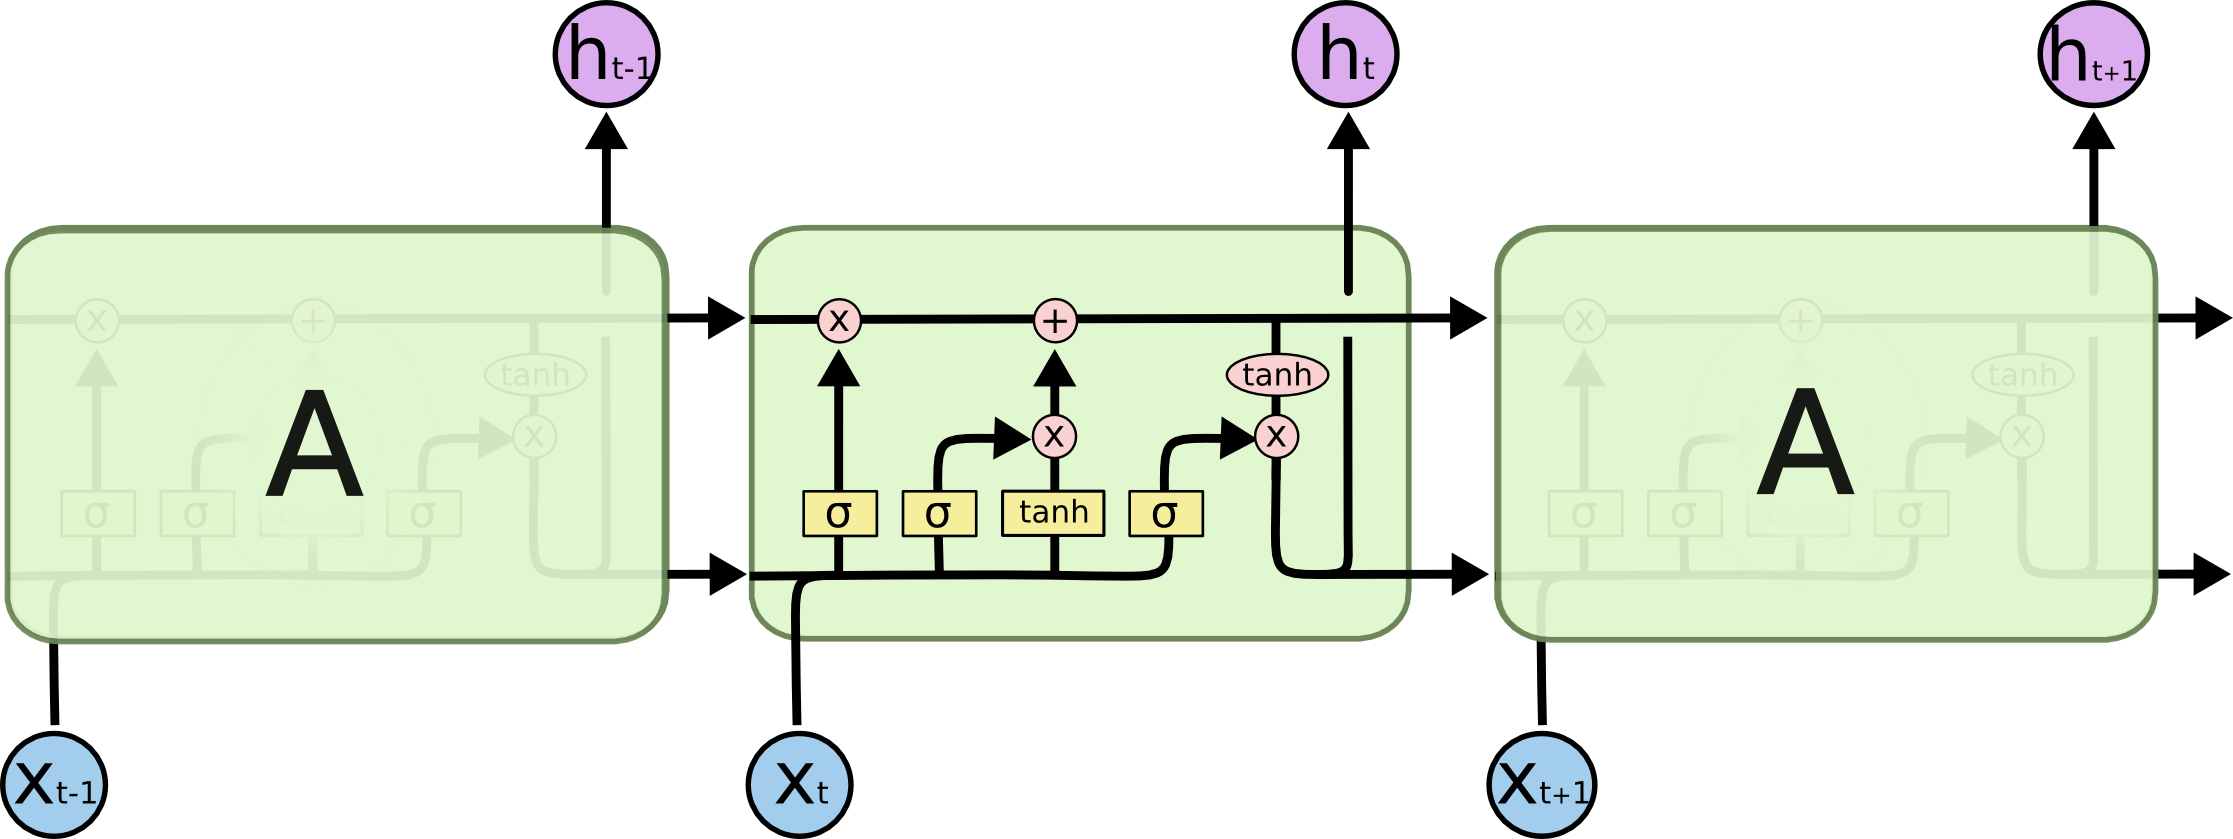
\includegraphics[width=0.8\linewidth]{img/lstm_chain.png}
  \caption{The repeating module in an LSTM}
  \label{fig:lstm_chain}
\end{figure}

In the diagram in figure \ref{fig:lstm_chain}, each line carries an entire vector, from the output of one node to the inputs of others.
The pink circles represent pointwise operations, like vector addition, while the yellow boxes are learned neural network layers.
Lines merging denote concatenation, while a line fork denotes its content being copied and the copies going to different locations.

\paragraph{The core idea behind LSTMs}

The key to LSTMs is the cell state, the horizontal line running through the top of the diagram.
The cell state is like a conveyor belt. It runs straight down the entire chain, with only some minor linear interactions.
It's very easy for information to just flow along it unchanged.

The LSTM does have the ability to remove or add information to the cell state, carefully regulated bu structures called gates.
Gates are a way to optionally let information through.
They are composed out of a sigmoid neural net layer and a pointwise multiplication operation.

The sigmoid layer outputs numbers between zero and one, describing how much of each component should be let through. A value of zero means "let nothing through", while a value of one means "let everything through".
An LSTM has three of these gates, to protect and control the cell state.

\paragraph{The four LSTM parts}
The first step in our LSTM is to decide what information we're going to throw away from the cell state.
This decision is made by a sigmoid layer called the "forget gate layer".
It looks at $h_{t-1}$ and $x_t$ and outputs a number between 0 and 1 for each number in the cell state $C_{t-1}$.
A 1 represents "remember this" while a 0 represents "forget this".

\begin{figure}[htbp]
  \centering
  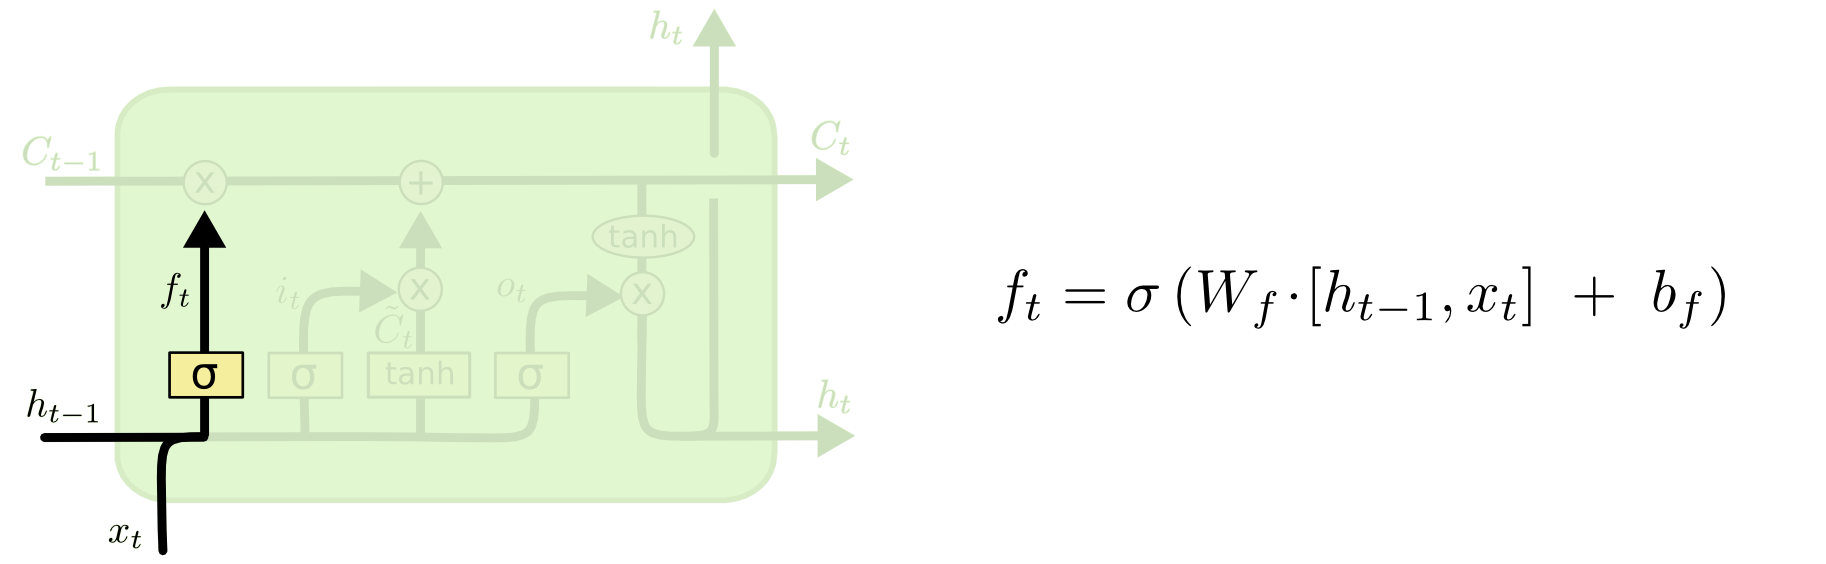
\includegraphics[width=0.6\linewidth]{img/lstm_forget.png}
  \caption{The forget module in an LSTM}
  \label{fig:lstm_forget}
\end{figure}

The next step is to decide what new information we're going to store in the cell state.
This has two parts.
First a sigmoid layer called the "input gate layer" decides which values we'll update.
Next, a tanh layer creates a vector of new candidate values, $\tilde{C}_t$, that could be added to the state.

\begin{figure}[htbp]
  \centering
  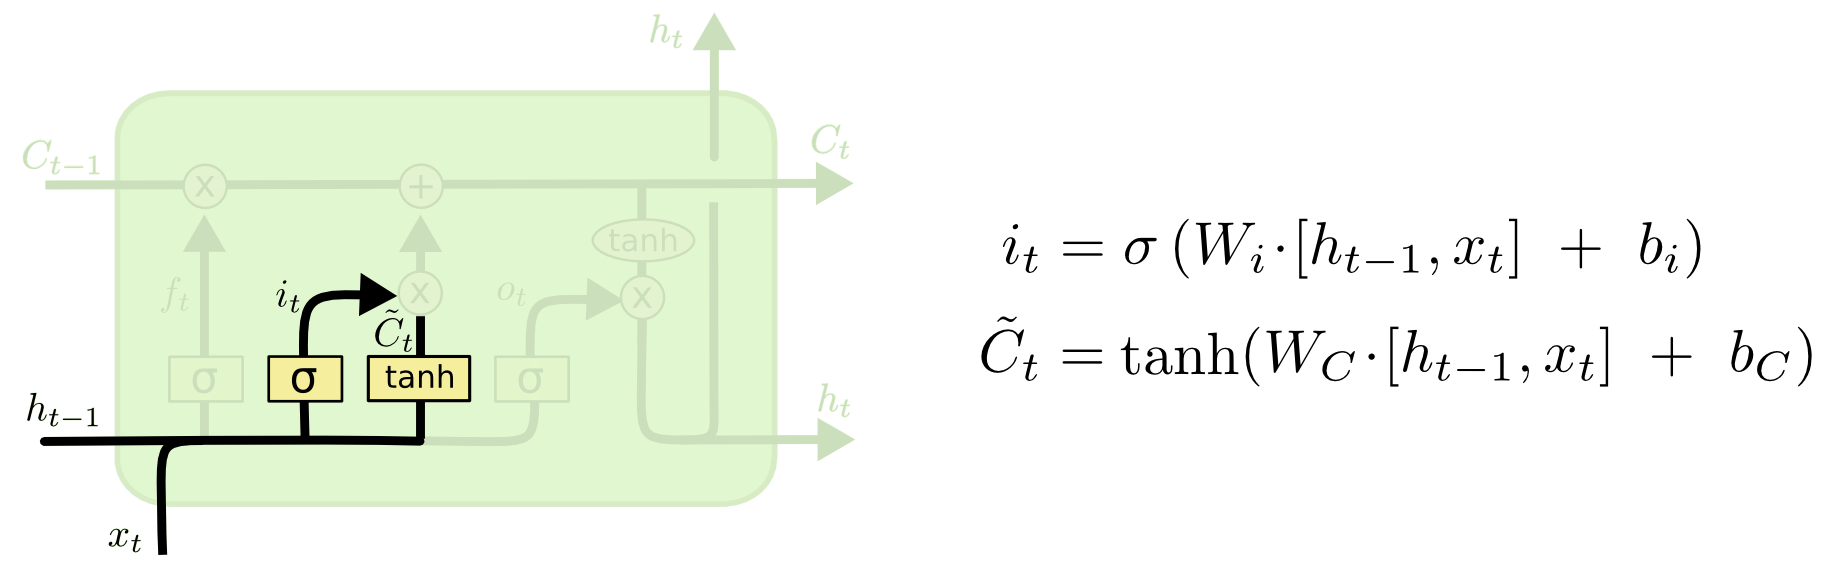
\includegraphics[width=0.6\linewidth]{img/lstm_input.png}
  \caption{The input module in an LSTM}
  \label{fig:lstm_input}
\end{figure}

Next, we have to update the old cell state $C_{t-1}$, into the new cell state $C_t$.
The previous steps already decided what to do, we just need to actually do it.
We multiply the old state by $f_t$, forgetting the things we decided to forget earlier.
Then we add $i_t * \tilde{C}_t$.
This is the new candidate values, scaled by how much we decided to update each state value.

\begin{figure}[htbp]
  \centering
  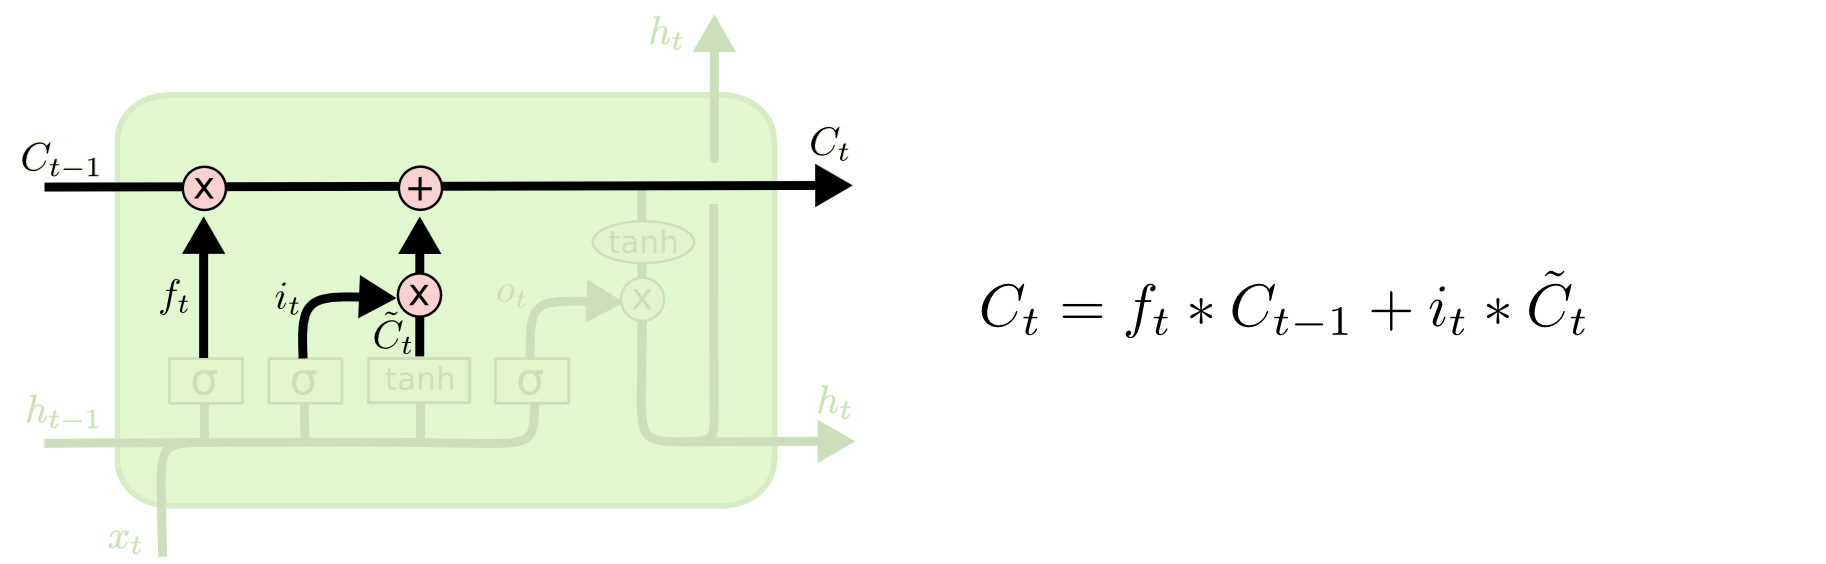
\includegraphics[width=0.6\linewidth]{img/lstm_update.png}
  \caption{The update module in an LSTM}
  \label{fig:lstm_update}
\end{figure}

Finally, we need to decide what we're going to output.
This output will be based on our cell state, but will be a filtered version.
First, we run a sigmoid layer which decides what parts of the cell sate we're going to output.
Then, we put the cell state through tanh (to push the values between -1 and 1) and multiply it by the output of the sigmoid gate, so that we only output the parts we decided to.

\begin{figure}[htbp]
  \centering
  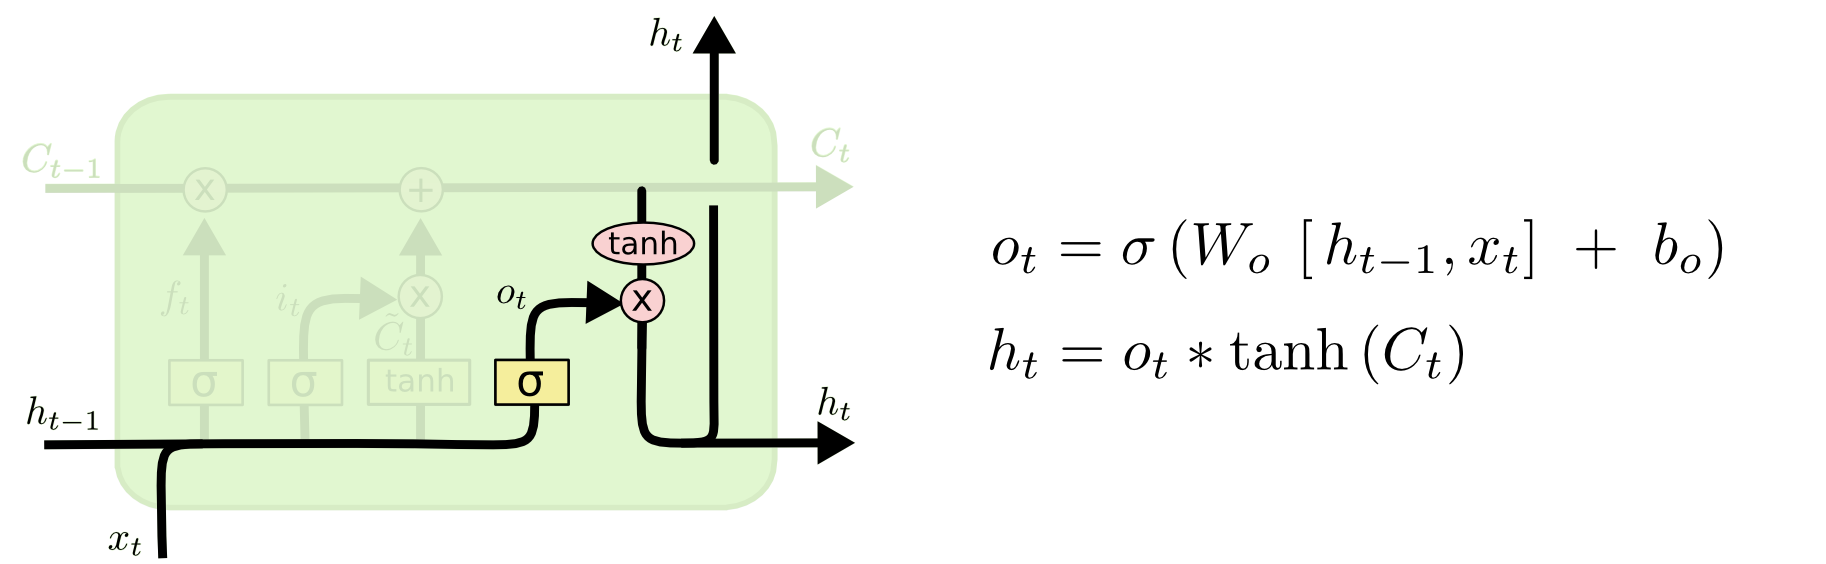
\includegraphics[width=0.6\linewidth]{img/lstm_output.png}
  \caption{The output module in an LSTM}
  \label{fig:lstm_output}
\end{figure}



\section{Technical implementation}

\subsection{Dataset}

The IMDB dataset is a widely used benchmark for sentiment analysis tasks.
It contains 50000 movie reviews from IMDB, allowing no more than 30 reviews per movie.
The dataset contains an even number of positive and negative reviews, so randomly guessing yields 50\% accuracy.
Also, neutral reviews are not included in the dataset \cite{imdb_dataset_stanfordnlp}.

\subsection{Data preprocessing}

The implementation includes several preprocessing steps.
The first one is data preprocessing.
Data preprocessing is important because raw textual data often contains noise, suck as typographical errors, inconsistent formatting and irrelevant symbols.
Preprocessing techniques aim to transform raw text data into a clean format that facilitates effective feature extraction and model training.

In this case I cleaned the dataset by removing: links, html tags, double spaces, punctuation and stopwords.
Stopwords are high frequency and low information words such as articles, prepositions, and conjunctions (e.g. "the", "and", "in") that are excluded to reduce noise and improve computational efficiency.
The stopwords were removed by using NLTK (Natural Language ToolKit), a suite of libraries and programs for natural language processing written in Python.
I also lemmatized the dataset.
Lemmatization is the process of reducing words to their root form, known as a lemma.
Unlike stemming, which simply chops off word endings, lemmatization considers the context and part of speech of a word to return a valid dictionary form (e.g. "running" is "run" and "better" is "good").
The entire dataset was also converted to lowercase.

We can see the dataset's head in the following code snippet:
\begin{itemize}
  \item Before the preprocessing:
    \begin{lstlisting}
    0      I rented I AM CURIOUS-YELLOW from my video sto...      0
    1      "I Am Curious: Yellow" is a risible and preten...      0
    2      If only to avoid making this type of film in t...      0
    3      This film was probably inspired by Godard's Ma...      0
    4      Oh, brother...after hearing about this ridicul...      0
    ...                                                  ...    ...
    49995  Just got around to seeing Monster Man yesterda...      1
    49996  I got this as part of a competition prize. I w...      1
    49997  I got Monster Man in a box set of three films ...      1
    49998  Five minutes in, i started to feel how naff th...      1
    49999  I caught this movie on the Sci-Fi channel rece...      1
    \end{lstlisting}

  \item After the preprocessing:
    \begin{lstlisting}
    0      rented curious yellow video store controversy ...      0
    1      curious yellow risible pretentious steaming pi...      0
    2      avoid making type film future film interesting...      0
    3      film probably inspired godard masculin feminin...      0
    4      oh brother hearing ridiculous film umpteen yea...      0
    ...                                                  ...    ...
    49995  got around seeing monster man yesterday long w...      1
    49996  got part competition prize watched really expe...      1
    49997  got monster man box set three film mainly want...      1
    49998  five minute started feel naff looking got comp...      1
    49999  caught movie sci fi channel recently actually ...      1
    \end{lstlisting}
\end{itemize}

\subsection{Model architectures}

% \section{Task description and data construction}
% \label{sec:headings}
% We are provided with five datasets from Kaggle: Sales train, Sale test, items, item categories and shops. In the Sales train dataset, it provides the information about the sales’ number of an item in a shop within a day. In the Sales test dataset, it provides the shop id and item id which are the items and shops we need to predict. In the other three datasets, we can get the information about item’s name and its category, and the shops’ name.
% \paragraph{Task modeling.}
% We approach this task as a regression problem. For every item and shop pair, we need to predict its next month sales(a number).
% \paragraph{Construct train and test data.}
% In the Sales train dataset, it only provides the sale within one day, but we need to predict the sale of next month. So we sum the day's sale into month's sale group by item, shop, date(within a month).
% In the Sales train dataset, it only contains two columns(item id and shop id). Because we need to provide the sales of next month, we add a date column for it, which stand for the date information of next month.

% \subsection{Headings: second level}
% \lipsum[5]
% \begin{equation}
% \xi _{ij}(t)=P(x_{t}=i,x_{t+1}=j|y,v,w;\theta)= {\frac {\alpha _{i}(t)a^{w_t}_{ij}\beta _{j}(t+1)b^{v_{t+1}}_{j}(y_{t+1})}{\sum _{i=1}^{N} \sum _{j=1}^{N} \alpha _{i}(t)a^{w_t}_{ij}\beta _{j}(t+1)b^{v_{t+1}}_{j}(y_{t+1})}}
% \end{equation}

% \subsubsection{Headings: third level}
% \lipsum[6]

% \paragraph{Paragraph}
% \lipsum[7]

% \section{Examples of citations, figures, tables, references}
% \label{sec:others}
% \lipsum[8] \cite{kour2014real,kour2014fast} and see \cite{hadash2018estimate}.

% The documentation for \verb+natbib+ may be found at
% \begin{center}
%   \url{http://mirrors.ctan.org/macros/latex/contrib/natbib/natnotes.pdf}
% \end{center}
% Of note is the command \verb+\citet+, which produces citations
% appropriate for use in inline text.  For example,
% \begin{verbatim}
%    \citet{hasselmo} investigated\dots
% \end{verbatim}
% produces
% \begin{quote}
%   Hasselmo, et al.\ (1995) investigated\dots
% \end{quote}

% \begin{center}
%   \url{https://www.ctan.org/pkg/booktabs}
% \end{center}


% \subsection{Figures}
% \lipsum[10] 
% See Figure \ref{fig:fig1}. Here is how you add footnotes. \footnote{Sample of the first footnote.}
% \lipsum[11] 

% \begin{figure}
%   \centering
%   \fbox{\rule[-.5cm]{4cm}{4cm} \rule[-.5cm]{4cm}{0cm}}
%   \caption{Sample figure caption.}
%   \label{fig:fig1}
% \end{figure}

% \begin{figure} % picture
%     \centering
%     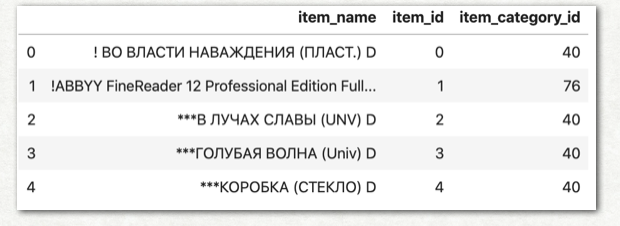
\includegraphics{test.png}
% \end{figure}

% \subsection{Tables}
% \lipsum[12]
% See awesome Table~\ref{tab:table}.

% \begin{table}
%  \caption{Sample table title}
%   \centering
%   \begin{tabular}{lll}
%     \toprule
%     \multicolumn{2}{c}{Part}                   \\
%     \cmidrule(r){1-2}
%     Name     & Description     & Size ($\mu$m) \\
%     \midrule
%     Dendrite & Input terminal  & $\sim$100     \\
%     Axon     & Output terminal & $\sim$10      \\
%     Soma     & Cell body       & up to $10^6$  \\
%     \bottomrule
%   \end{tabular}
%   \label{tab:table}
% \end{table}

% \subsection{Lists}
% \begin{itemize}
% \item Lorem ipsum dolor sit amet
% \item consectetur adipiscing elit. 
% \item Aliquam dignissim blandit est, in dictum tortor gravida eget. In ac rutrum magna.
% \end{itemize}


\bibliographystyle{unsrt}

% Remove comment to use the external .bib file (using bibtex).
\bibliography{references.bib}
% and comment out the ``thebibliography'' section.


% %%% Comment out this section when you \bibliography{references} is enabled.
% \begin{thebibliography}{1}

% \bibitem{kour2014real}
% George Kour and Raid Saabne.
% \newblock Real-time segmentation of on-line handwritten arabic script.
% \newblock In {\em Frontiers in Handwriting Recognition (ICFHR), 2014 14th
%   International Conference on}, pages 417--422. IEEE, 2014.

% \bibitem{kour2014fast}
% George Kour and Raid Saabne.
% \newblock Fast classification of handwritten on-line arabic characters.
% \newblock In {\em Soft Computing and Pattern Recognition (SoCPaR), 2014 6th
%   International Conference of}, pages 312--318. IEEE, 2014.

% \bibitem{hadash2018estimate}
% Guy Hadash, Einat Kermany, Boaz Carmeli, Ofer Lavi, George Kour, and Alon
%   Jacovi.
% \newblock Estimate and replace: A novel approach to integrating deep neural
%   networks with existing applications.
% \newblock {\em arXiv preprint arXiv:1804.09028}, 2018.

% \end{thebibliography}


\end{document}
